%%%%%%%%%%%%%%%%%%%%
%%%% FORMATTING %%%%
%%%%%%%%%%%%%%%%%%%%
\documentclass[11pt,a4paper]{article}  % Set the class of the document to article with 10pt font size and A4 paper size
\setlength{\textheight}{25.7cm}  % Set the height of the text area to 25.7cm
\setlength{\textwidth}{16cm}  % Set the width of the text area to 16cm
\setlength{\unitlength}{1mm}  % Set the default unit length for picture environments to 1mm
\setlength{\topskip}{2truecm}  % Set the skip above the top baseline of the text area to 2cm
% Calculate and set the top margin
\topmargin 260mm \advance \topmargin -\textheight 
\divide \topmargin by 2 \advance \topmargin -1in 
% Set the header height and separation to 0pt
\headheight 0pt
\headsep 0pt
% Calculate and set the left margin
\leftmargin 210mm \advance \leftmargin -\textwidth 
\divide \leftmargin by 2 \advance \leftmargin -1in 
% Set the odd and even side margins to the calculated left margin
\oddsidemargin \leftmargin
\evensidemargin \leftmargin
% Set the paragraph indentation to 0pt
\parindent=0pt
% Formatting of (sub)section headers
\usepackage[medium]{titlesec}
\titlespacing\section{0pt}{12pt plus 4pt minus 2pt}{0pt plus 2pt minus 2pt}
\titlespacing\subsection{0pt}{12pt plus 4pt minus 2pt}{0pt plus 2pt minus 2pt}
\titlespacing\subsubsection{0pt}{12pt plus 4pt minus 2pt}{0pt plus 2pt minus 2pt}
% Paragraph formatting
\setlength{\parindent}{0ex}  % Removes default indent at new paragraph
\setlength{\parskip}{.5em}  % Sets the vertical space between two paragraphs.
% Move down page numbers
\setlength{\footskip}{2cm} 
% Include subsubsections in table of contents
\setcounter{tocdepth}{3}


%%%%%%%%%%%%%%%%%%
%%%% PACKAGES %%%%
%%%%%%%%%%%%%%%%%%
\usepackage{tikz}
\usepackage[toc, page]{appendix}  % For adding appendices.
\usepackage[english]{babel}  % Provides multilingual support for LaTeX documents.
\usepackage[format=plain, font=it]{caption}  % Customizes the formatting of captions for figures and tables.
\usepackage[utf8]{inputenc}  % Specifies the input encoding of the document to UTF-8, allowing for the direct input of special characters.
\usepackage{amssymb}  % Provides access to various mathematical symbols and fonts.
% \usepackage{commath}  % Offers additional mathematical commands and environments for typesetting mathematical expressions.
\usepackage{mathtools}  % Enhances the functionality of mathematical typesetting, providing additional tools and symbols for mathematical equations.
\usepackage[shortlabels]{enumitem}  % Customizes the appearance and behavior of lists, allowing for different label styles and formatting options.
\usepackage{gensymb}  % Provides access to generic symbols, including common symbols like degree symbol (°).
\usepackage{calligra}  % Allows the use of the calligraphic font style in the document.
\usepackage{amsmath}  % Enhances the functionality of mathematical typesetting in LaTeX.
\usepackage[hidelinks]{hyperref}  % Enables the creation of hyperlinks within the document, with the hidelinks option used to hide the colored boxes around hyperlinks.
\usepackage{wrapfig}  % Facilitates the wrapping of text around figures or tables.
\usepackage{booktabs}  % Enhances the quality of tables by providing guidelines for proper table formatting.
\usepackage{multicol}  % Enables the creation of multi-column layouts in the document.
\usepackage{multirow}  % Allows for the merging of rows in tables.
\usepackage{ctable}  % Provides customizable tables with improved features compared to standard LaTeX tables.
\usepackage{subcaption}  % Enhances the functionality of subcaptions for subfigures and subtables.
\usepackage{systeme}  % Aids in the typesetting of systems of equations.
\usepackage{lipsum}  % Generates dummy text (lorem ipsum) for testing the layout and formatting of the document.
\usepackage{tocloft}  % Allows for the customization of table of contents formatting.
\usepackage{secdot}  % Adds a dot after section numbers in the document.
\usepackage{dirtytalk}  % Typeset quotations with proper quotation marks
\usepackage{systeme}  % For systems of equations 
\usepackage{esint}  % Nice looking integrals
\usepackage{enumitem}  % Offers more flexibility for lists
\usepackage{wrapfig}  % Wrap text around figures


% Style for code using listings
\usepackage{listings}
\usepackage{xcolor}

\definecolor{codegreen}{rgb}{0,0.6,0}
\definecolor{codegray}{rgb}{0.5,0.5,0.5}
\definecolor{codepurple}{rgb}{0.58,0,0.82}
\definecolor{backcolour}{rgb}{0.95,0.95,0.92}
\lstdefinestyle{mystyle}{
	backgroundcolor=\color{backcolour},   
	commentstyle=\color{codegreen},
	keywordstyle=\color{magenta},
	numberstyle=\tiny\color{codegray},
	stringstyle=\color{codepurple},
	basicstyle=\ttfamily\footnotesize,
	breakatwhitespace=false,         
	breaklines=true,                 
	captionpos=b,                    
	keepspaces=true,                 
	numbers=left,                    
	numbersep=5pt,                  
	showspaces=false,                
	showstringspaces=false,
	showtabs=false,                  
	tabsize=2
}
\lstset{style=mystyle}


% Set colors for citation numbers, equation numbers, links and URLs
% Blue citation numbers
% Magenta links (e.g. in table of contents)
% Red equation numbers
\hypersetup{colorlinks, linkcolor={black}, citecolor={blue}, urlcolor={magenta}} 
\renewcommand\theequation{{\color{red}\arabic{equation}}} 

% Symbols for footnotes
\usepackage[symbol]{footmisc}
\renewcommand{\thefootnote}{\fnsymbol{footnote}}

% Table and Figure captions formatting
\usepackage[font={sl}, format = hang, labelfont=bf]{caption}  


%%%%%%%%%%%%%%%%%%
%%%% COMMANDS %%%%
%%%%%%%%%%%%%%%%%%
\renewcommand{\d}[1]{\ensuremath{\operatorname{d}\!{#1}}} % \d command for upright d in differentials. Also has some space before it for at the end of an integral.
\newcommand{\angstrom}{\text{\normalfont\AA}}  % \angstrom argument for angstrom symbol
% Below is for recreating the script-r from Griffith's "Introduction to Electrodynamics".
% Use \scripty{r} as command. Can also be made bold or given a hat.
\DeclareMathAlphabet{\mathcalligra}{T1}{calligra}{m}{n}
\DeclareFontShape{T1}{calligra}{m}{n}{<->s*[2.2]callig15}{}
\newcommand{\scripty}[1]{\ensuremath{\mathcalligra{#1}}}  


%%% Color boxex for "Optional" and "Example" parts.
\usepackage{tcolorbox}
\tcbuselibrary{skins, breakable}
\definecolor{darkblue}{RGB}{0, 0, 139}
\definecolor{darkgreen}{RGB}{0, 80, 0}
\definecolor{warningorange}{HTML}{B06000}

\newtcolorbox{optionalbox}[1][]{
	breakable,
	enhanced,
	colback=gray!8,
	colframe=gray!50,
	colupper=darkblue,
	fontupper=\normalfont,
	fonttitle=\bfseries\color{darkblue},
	title=Optional,
	attach boxed title to top left={yshift=-2mm, xshift=4mm},
	boxed title style={colback=white, colframe=gray!50},
	#1
}

\newtcolorbox{examplebox}[1][]{
	breakable,
	enhanced,
	colback=gray!8,
	colframe=gray!50,
	colupper=darkgreen,
	fontupper=\normalfont,
	fonttitle=\bfseries\color{darkgreen},
	title=Example,
	attach boxed title to top left={yshift=-2mm, xshift=4mm},
	boxed title style={colback=white, colframe=gray!50},
	#1
}


\usepackage{menukeys}

\usepackage{graphicx}
\usepackage{array}
\usepackage{longtable}
\usepackage{makecell}

\usepackage{xstring}
\graphicspath{ {./images/} }

\newread\GlycoDashDescriptionFile
\newcommand{\GlycoDashVersion}{unknown}
\newcommand{\ReadGlycoDashVersion}[1]{%
	\openin\GlycoDashDescriptionFile=#1\relax
	\ifeof\GlycoDashDescriptionFile
	\else
		\loop\unless\ifeof\GlycoDashDescriptionFile
			\read\GlycoDashDescriptionFile to \GlycoDashDescriptionLine
			\IfBeginWith{\GlycoDashDescriptionLine}{Version: }{%
				\StrBehind{\GlycoDashDescriptionLine}{Version: }[\GlycoDashVersion]%
			}{}%
		\repeat
	\fi
	\closein\GlycoDashDescriptionFile
}
\ReadGlycoDashVersion{../../DESCRIPTION}
\IfStrEq{\GlycoDashVersion}{unknown}{\ReadGlycoDashVersion{DESCRIPTION}}{}

\begin{document}
	% Title page
	\begin{titlepage}
		\centering
		\vspace*{1cm}
		
		% Title
		\scalebox{2.5}{\Huge\textbf{GlycoDash}}
		\vspace{0.5cm}
		
		% Subtitle
		{\Huge \textbf{User Guide}}
		
		% Logo
		\vspace{2.5cm}
		
\includegraphics[scale = 0.45]{logo.png}
		
		
		\vfill
		% Version text
		{\Huge \textit{Version \GlycoDashVersion}}
		
	\end{titlepage}
	
	% Table of contents
	\newpage
	\tableofcontents
	
	% Sections
	\graphicspath{ {./images/1_Overview} }
\newpage

\section{Overview}
\subsection{Background}
GlycoDash is an R Shiny dashboard created for processing mass spectrometry data obtained from LaCyTools, SweetSuite or Skyline.
The data is uploaded to the dashboard and optionally merged with metadata.
Spectral curation and analyte curation are then performed to exclude data that is of insufficient quality from further analysis.
Total area normalization is performed on the curated glycopeptide data per glycosylation site.
GlycoDash then offers the options to calculate glycosylation traits, quantify proteins, determine glycosylation site occupancies, assess the repeatability of technical replicates, and to perform simple data visualizations.

The output data is a file in \texttt{.xlsx} format that can be easily imported into software such as RStudio or SPSS for further data analysis.
A processing report in HTML format can also be downloaded.
By listing all choices that were made, this file ensures the reproducibility of all processing steps.

For background information about GlycoDash, please refer to \href{https://doi.org/10.1007/s00216-025-05794-3}{our publication}.
GlycoDash has undergone continued development and refinement since this paper was published.
The current version includes additional features and improvements that extend beyond the scope of the published manuscript.


\subsection{User interface}
When launching GlycoDash, you will be presented with the page shown below. 

\begin{center}
	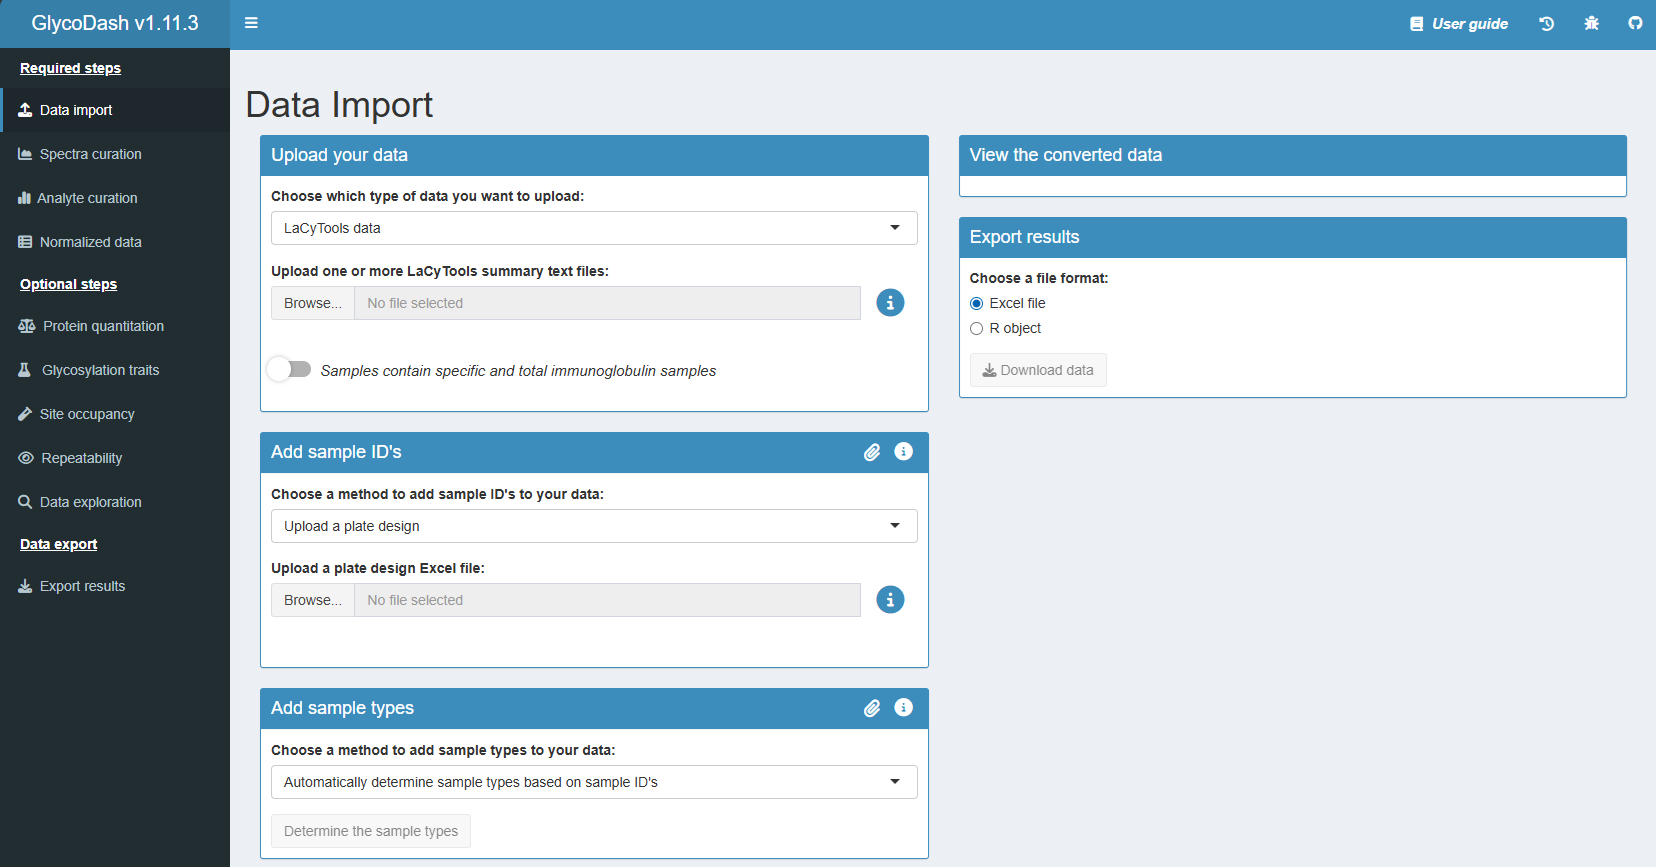
\includegraphics[scale=0.35]{interface.png}
\end{center}

The top-left corner displays the version number of GlycoDash.
The left column contains various tabs. 
The first four tabs (\menu{Data import}, \menu{Spectra curation}, \menu{Analyte curation} and \menu{Normalized data}) should be completed in the listed order, as detailed in subsequent sections. 
Later tabs are optional and can be skipped. 
The buttons in the top-right corner can be used to download the latest version of the user guide, to download a changelog, to view a list of known bugs and issues, or to visit the \href{https://github.com/Center-for-Proteomics-and-Metabolomics/GlycoDash}{GitHub page} containing the source code of GlycoDash.

	\graphicspath{ {./images/2_Data_import} }
\newpage

\section{Data import}\label{data_import}
\subsection{Raw data input}
In the \textsf{Upload your data} box, choose the type of raw data that you want to upload: LaCyTools data, Skyline data or SweetSuite data. 
Hovering over the blue info icon will show information about the formatting requirements. 
See the sections below for more details.

The uploaded data is converted into a clean data frame, with a column for each variable in the data.
The converted data is displayed in the top-right box \textsf{View the converted data} in the dashboard.

\begin{optionalbox}
	When applicable, specify keywords by which total and specific immunoglobulin samples can be recognized in the sample names.
	The specification is case sensitive.
	The table with converted data will be given an additional column called \textsf{group}, specifying whether a sample contains total or specific glycosylation data.
	Total and specific samples will be curated separately in later steps.
	\begin{center}
		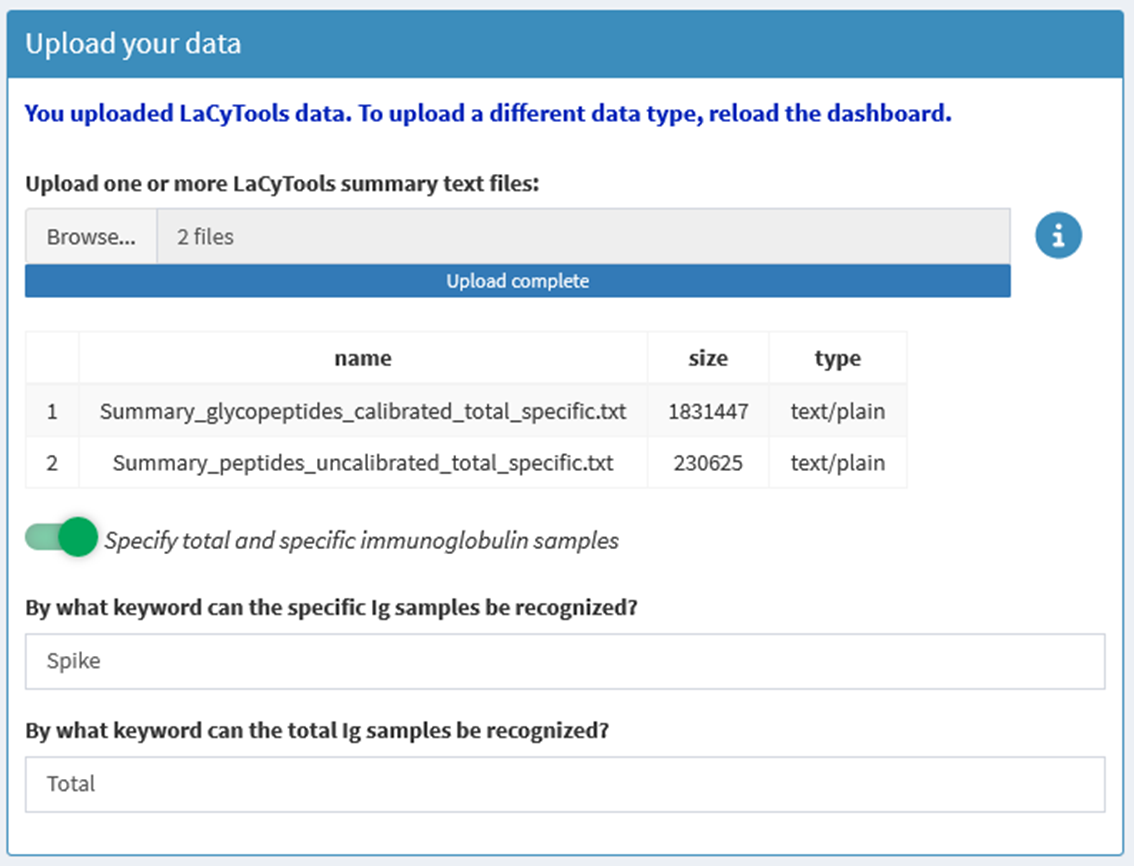
\includegraphics[width=0.62\linewidth]{import_lacytools.png}
	\end{center}
\end{optionalbox}

\subsubsection{Formatting of LaCyTools data}
You can upload one or more summary text files created by LaCyTools. 
The names and sizes of the uploaded files will be displayed in a table.
Each LaCyTools summary text file must contain at least the following outputs:

\begin{enumerate}[topsep=0pt, itemsep=0pt]
	\item Background subtracted absolute intensity
	\item Mass accuracy (ppm)
	\item Isotopic pattern quality (IPQ)
	\item Signal-to-noise ratio ($S/N$)
\end{enumerate}

These outputs should be present for each analyte, per charge state.

\subsubsection{Formatting of SweetSuite data}
SweetSuite creates an \texttt{.xlsx} file as output.
The \textsf{Data} sheet in this file contains several columns by default.
These \texttt{.xlsx} files can be uploaded directly into GlycoDash.

It is possible to upload multiple files at once.


\newpage
\subsubsection{Formatting of Skyline data (wide format)}
You can upload one \texttt{.csv} output file from Skyline.
The required formatting of the file depend on the way in which analytes are specified.
Analytes (glycopeptides) in the file must be specified in \emph{one of two ways}:

\begin{enumerate}[topsep=0pt, itemsep=0pt]
	% One column
	\item 
	\textbf{One column} where each entry contains both a peptide sequence and a glycan composition, e.g. \textsf{EEQYN[H3N4F1]STYR}.
	This column will likely be called either \textsf{Peptide Modified Sequence Full Names} or \textsf{Peptide Modified Sequence Three Letter Codes}.
	A sequence in this column may also contain methionine oxidation and cysteine carbamidomethyl (CAM) modifications.
	These modifications may be fully written out (\textsf{[Oxidation (M)], [Carbamidomethyl (C)]}), or they can be specified using a three letter abbreviation (\textsf{[Oxi], [CAM]}).
	\emph{Other modifications are currently not supported.}
	
	There must also be column containing protein names and a column specifying the charge states of the analytes.
	These columns will likely be called \textsf{Protein Name} and \textsf{Precursor Charge}, respectively.
	Additionally, the file should contains columns with \textsf{Total Area MS1}, \textsf{Isotope Dot Product} and \textsf{Average Mass Error PPM} \emph{for each sample name}.
	
	In the user interface, select the required columns and press the \menu{Process skyline data} button.
	
	Each unique combination of protein name and peptide sequence will be assigned a unique glycosylation site.
	The protein names will be converted to \textsf{PrA}, \textsf{PrB}, etc. in alphabetical order. 
	Peptide sequences will be abbreviated using the first three letters of the sequence. 
	When two or more peptides in a protein share the first three sequence letters, suffices (\textsf{\_a}, \textsf{\_b}, \textsf{\_c} etc.) are added to the sequence abbreviation.
	Finally, the protein and sequence abbreviations are pasted together with an underscore separating them, to form a string representing a unique glycosylation site.
	A downloadable table is generated where the protein names and peptide sequences can be linked to the assigned glycosylation sites. 
	
	\begin{center}
		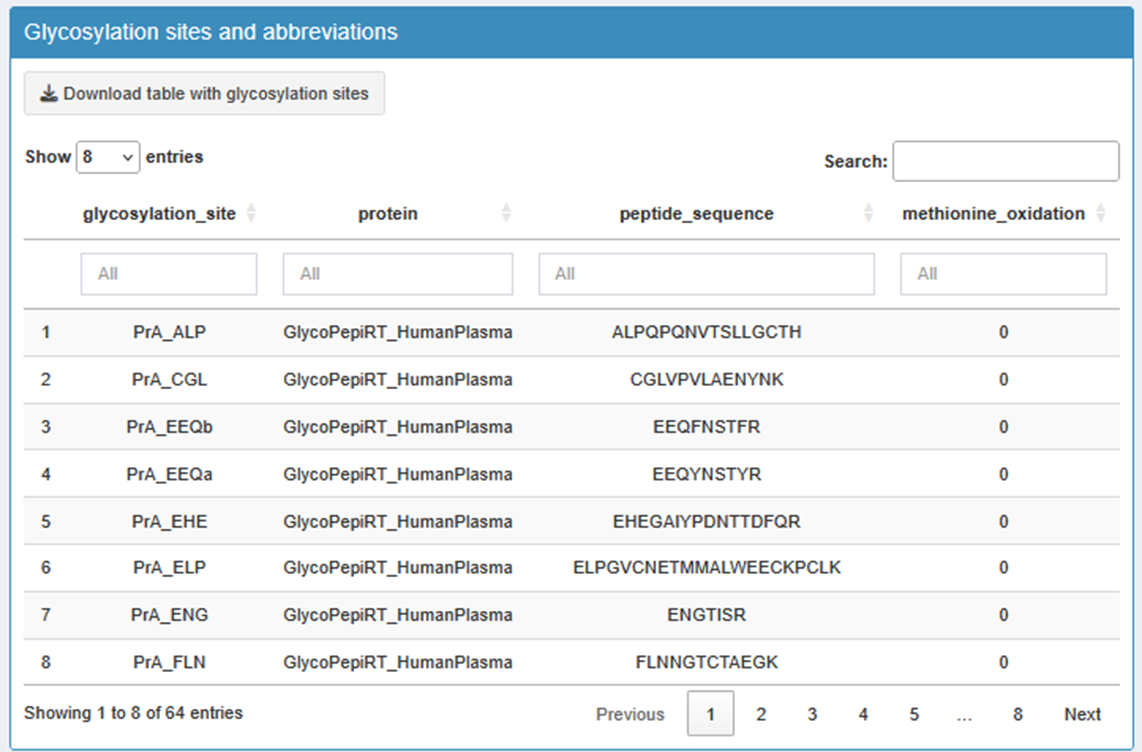
\includegraphics[scale=0.45]{skyline_peptides_table.png}
	\end{center}
	
	The column \textsf{methionine\_oxidation} lists the number of oxidized methionine residues in the corresponding peptide sequence.
	For each oxidized methionine, the \textsf{glycosylation\_site} entry is given an extra suffix \textsf{Ox}.
	
	% Two columns
	\item 
	\textbf{Two columns}, one with glycosylation sites and one containing glycan compositions.
	The glycosylation sites and glycans will be combined into a single analyte name (e.g., glycosylation site \textsf{PepI} and glycan \textsf{H3N4F1} will be combined into analyte \textsf{PepI1H3N4F1}).
	When analytes are specified this way, there must also be a column specifying the charge states of the analytes.
	This column will likely be called \textsf{Precursor Charge}.
	
	Additionally, the file should contain columns with \textsf{Total Area MS1}, \textsf{Isotope Dot Product} and \textsf{Average Mass Error PPM} \emph{for each sample name}.
	
	In the user interface, select the required columns and press \menu{Process skyline data} button.
		
\end{enumerate}


\begin{optionalbox}
	Skyline data may contain a column with notes for each analyte. 
	This column is likely called \textsf{Peptide Note}.
	After toggling the option \menu{Specify column with analyte notes} and selecting the corresponding column, an extra tab with notes for each analyte will be added to the output \texttt{.xlsx} file when exporting the processed data.
\end{optionalbox}

By default, analytes with isomeric glycan compositions are automatically detected and renamed when processing Skyline data.
For example, when \textsf{PepIH5N2} is present twice per sample (in each charge state), they are renamed to \textsf{PepIH5N2\_a} and \textsf{PepIH5N2\_b}. 
This renaming of isomers can be prevented by unchecking \menu{Automatically detect and rename glycan isomers}.



\subsubsection{Adding sample IDs}
Choose a method by which to add sample IDs:
\begin{itemize}[topsep=0pt, itemsep=0pt]
	\item 
	\textsf{Upload a plate design}  - This method requires each sample name to include a plate number and well position separated by an underscore. Examples of correctly formatted sample names are \textsf{MS\_\textbf{PL01\_B09}\_01\_2020.raw} and \textsf{IM1\_\textbf{PL02\_A11}\_03}.

	The plate design should be in \texttt{.xlsx} format, with different plates separated by an empty row.
	Each cell in the plate layout should contain a sample ID for the corresponding sample.
	If a plate well was not measured, the corresponding cell can be empty.
	Duplicate sample IDs are allowed to be present.
	An example of a plate design can be downloaded by clicking on the paperclip icon in the top-right corner of the \textsf{Add sample IDs} box.
	
	\begin{optionalbox}
		When applicable, you can upload separate plate layouts for total and specific immunoglobulin samples.
	\end{optionalbox}
	
	
	\item 
	\textsf{Upload a sample list} - Use this method when your sample names do not follow previously described format.
	The sample list should be a file in \texttt{.xlsx} format with the following two columns:
	\begin{enumerate}[topsep=0pt, itemsep=0pt]
		\item 
		\textsf{sample\_name} - This column should contain all the sample names that are present in the data (matching the names in the first column of the converted data).
		\item
		\textsf{sample\_id} - This column should contain the sample IDs corresponding to each sample name (e.g., \textsf{blank}, \textsf{pool}, \textsf{plasma}).
	\end{enumerate}
	An example of a sample list can be downloaded by clicking on the paperclip icon the top-right corner of the \textsf{Add sample IDs} box.
	
\end{itemize}

After uploading the required \texttt{.xlsx} file, a \textsf{sample\_id} column is automatically added to the converted data.


\newpage
\subsubsection{Adding sample types}
First choose a method to add sample types:
\begin{itemize}[topsep=0pt, itemsep=0pt]
	\item
	\textsf{Automatically} - Sample types are identified by finding common text patterns shared across sample IDs.
	For example, sample IDs \textsf{standard\_1} and \textsf{standard\_2} would both be assigned the sample type \textsf{standard}.
	\item 
	\textsf{Upload a list with sample types} - The uploaded list should a \texttt{.xlsx} file with two columns:
	\begin{itemize}[topsep=0pt, itemsep=0pt]
		\item 
		\textsf{sample\_id} - This column should contain each sample ID once (even if a sample ID appears multiple times in your data).
		\item 
		\textsf{sample\_type} - This column should specify the sample type corresponding to each sample ID.
		For instance, sample ID \textsf{PBS} could be assigned the sample type \textsf{blank}.
		Sample IDs \textsf{standard\_1} and \textsf{standard\_2} could be assigned the sample type \textsf{standard}.
		An example sample type file can be downloaded by clicking the paperclip button in the \textsf{Add sample types} box.
	\end{itemize}
\end{itemize}

Then, depending on your chosen method of adding sample types:
\begin{itemize}[topsep=0pt, itemsep=0pt]
	\item 
	\textsf{Automatically} - Click the \menu{Determine the sample types} button.
	A popup is shown with the detected sample types.
	To use these detected sample types, \menu{Accept these sample types}.
	If you want to use the other method instead, click \menu{Cancel}.
	\item 
	\textsf{Upload a list with sample types} - Upload your \texttt{.xlsx} file.
	The sample types will be added to the data automatically.
\end{itemize}


\subsubsection{Detection of glycosylation sites}
Glycopeptides in the data will automatically be assigned to glycosylation sites based on their names.
For example, two analytes \textsf{IgGI1H3N4F1} and \textsf{IgGI1H4N4F1} would both be assigned to the same glycosylation site \textsf{IgGI}.
Spectra curation and analyte curation will later be performed per glycosylation site.

\begin{optionalbox}
	Your data may contain heavy isotope labeled glycopeptides, such as SILuMAb IgG1 glycopeptides.
	These labeled glycopeptides will be assigned to glycosylation sites that are distinct from their natural counterparts.
\end{optionalbox}

Non-glycosylated peptides in your data are automatically detected. Two situations can occur:

\begin{itemize}[topsep=0pt, itemsep=0pt]
	\item 
	When there are glycopeptides whose glycosylation site corresponds to a non-glycosylated peptide, then this peptide can later be used for calculating site occupancies. 
	For example, if the analyte \textsf{IgGI1} is present in the the data, then this can be used to calculate the occupancy of glycosylation site \textsf{IgGI}.
	\item 
	When no corresponding glycopeptides exist in your data, then the non-glycosylated peptide is assumed to not be derived from a glycosylation site.
	These peptides can later be used for protein quantitation.
\end{itemize}
	

\subsubsection{Adding metadata (optional)}
You can upload a \texttt{.xlsx} file containing metadata such as age, sex and disease status.
This data will be merged with the glycosylation data.
This integration ensures that the final output data is ready for further data analysis in a program of your choice.
The metadata can later also be used to perform analyte curation per biological group.
The \texttt{.xlsx} file must contain one column with sample IDs, and additional columns with the metadata.






	\graphicspath{ {./images/3_Spectra_curation} }
\newpage

\section{Spectra curation}
\subsection{Choosing analyte quality criteria}
The analyte quality criteria are used to judge whether the signal of an analyte is of sufficient quality in a given sample to be reliably quantified.
It is important to note that different charge states for the same glycopeptide are treated as distinct analytes. 
This information is used for spectra curation and for the subsequent analyte curation step. 
Depending on the type of data uploaded, there are three distinct quality criteria for which boundaries can be configured.
An analyte is deemed to be of sufficient quality when it meets all three criteria. 
Only in very specific cases, one or two of the listed quality criteria may be used, by clicking the gears icon and deselecting the criteria that you wish to ignore.

\subsubsection{LaCyTools or SweetSuite data}
\begin{wrapfigure}{R}{0.37\textwidth}
	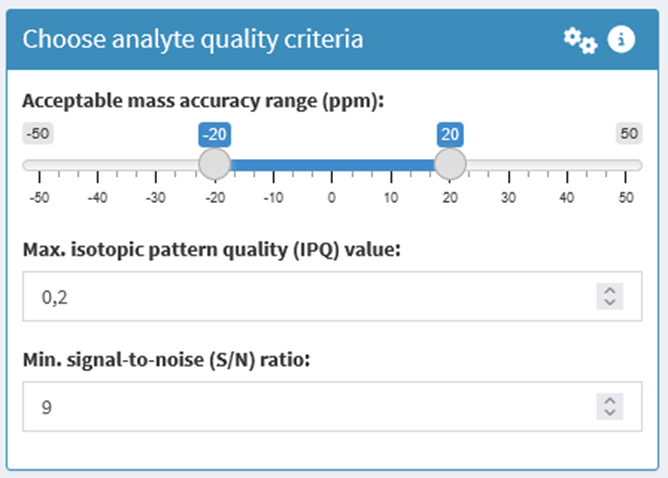
\includegraphics[scale = 0.35]{qc1.png}
 \end{wrapfigure}
Three quality criteria can be set for LaCyTools and SweetSuite data:

\begin{itemize}[topsep=0pt, itemsep=0pt]
	\item \textsf{Acceptable mass accuracy range (ppm)} \\
	Sets the acceptable mass accuracy (mass error) in parts-per-million (ppm).
	The maximum range is $-50$ to $+50$ ppm, with the default being $-20$ to $+20$ ppm.
	\item \textsf{Maximum isotopic pattern quality (IPQ) value} \\
	Sets the maximum acceptable IPQ value for an analyte.
	The lower the IPQ value of an analyte, the better the observed isotopic pattern of that analyte matches the theoretical isotopic pattern.
	The default value is $0.2$.
	\item \textsf{Maximum signal-to-noise ($S/N$) ratio} \\
	The minimum $S/N$ ratio that an analyte should have to be considered of sufficient quality.
	The default value is $9$.
\end{itemize}


\subsubsection{Skyline data}
\begin{wrapfigure}{R}{0.37\textwidth}
	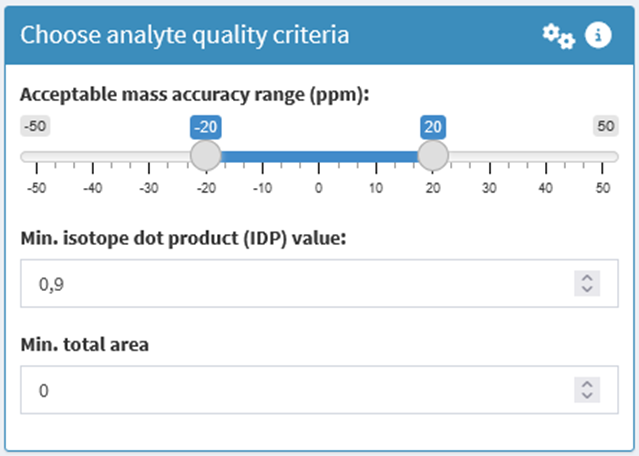
\includegraphics[scale = 0.35]{qc2.png}
\end{wrapfigure}
Three quality criteria can be set for Skyline data:

\begin{itemize}[topsep=0pt, itemsep=0pt]
	\item \textsf{Acceptable mass accuracy range (ppm)} \\
	Sets the acceptable mass accuracy (mass error) in parts-per-million (ppm).
	The maximum range is $-50$ to $+50$ ppm, with the default being $-20$ to $+20$ ppm.
	\item \textsf{Minimum isotope dot product (IDP) value} \\
	The minimum IDP value that an analyte should have.
	The higher the IDP value, the better the observed isotopic pattern of an analyte matches its theoretical isotopic pattern.
	The IDP can have a maximum value of 1, indicating a perfect match.
	The default minimum value is set to $0.9$.
	\item \textsf{Minimum total area} \\
	As Skyline does not output $S/N$ values, the total area can be used as an alternative.
	By default, this values is set to 0 (i.e. it is ignored).
\end{itemize}


\newpage
\subsection{Spectra curation cut-offs}
For each sample and glycosylation site in your data, the intensities of all analytes fulfilling the set QC parameters are summed, and the percentage of passing analytes out of all targeted analytes is calculated. 
Each spectrum will be curated based on these values. 
The two available methods for curating the spectra are described below.
Alternatively, you have the option to skip spectra curation, in which case all spectra will be utilized in subsequent processing steps.

\subsubsection{Curate spectra based on negative controls}
First, choose which sample types should be used as negative controls.
Then set a percentile of negative control measurements for calculating cut-off values.
The default percentile is set to 95.
Cut-off values will be computed for both the ``sum intensity'' and ``percentage of passing analytes'' values.
These cut-offs are calculated separately for each glycosylation site.

\begin{optionalbox}
	By default, uncalibrated spectra are treated as having missing values and will be excluded from the calculations.
	It is possible to include them with a value of zero by unchecking the \menu{Treat uncalibrated spectra as missing values, not zeros} option.
\end{optionalbox}

During curation, spectra whose percentage of passing analytes and sum intensity exceed or equal the corresponding cut-off values will pass curation.
These passing spectra will be used for further data processing.
In the \textsf{Perform spectra curation} box, all spectra are displayed per glycosylation site in an interactive plot, color-coded by sample type.
The cut-off values are indicated by dashed bars, and the exact cut-off values are displayed below the plot.

When satisfied with the cut-off values, click on \menu{Perform spectra curation}

\begin{optionalbox}
	It is possible to set manual cut-offs for a glycosylation site by toggling the \menu{\textsf{Set cut-offs manually}} option in the corresponding tab.
\end{optionalbox}

\begin{center}
	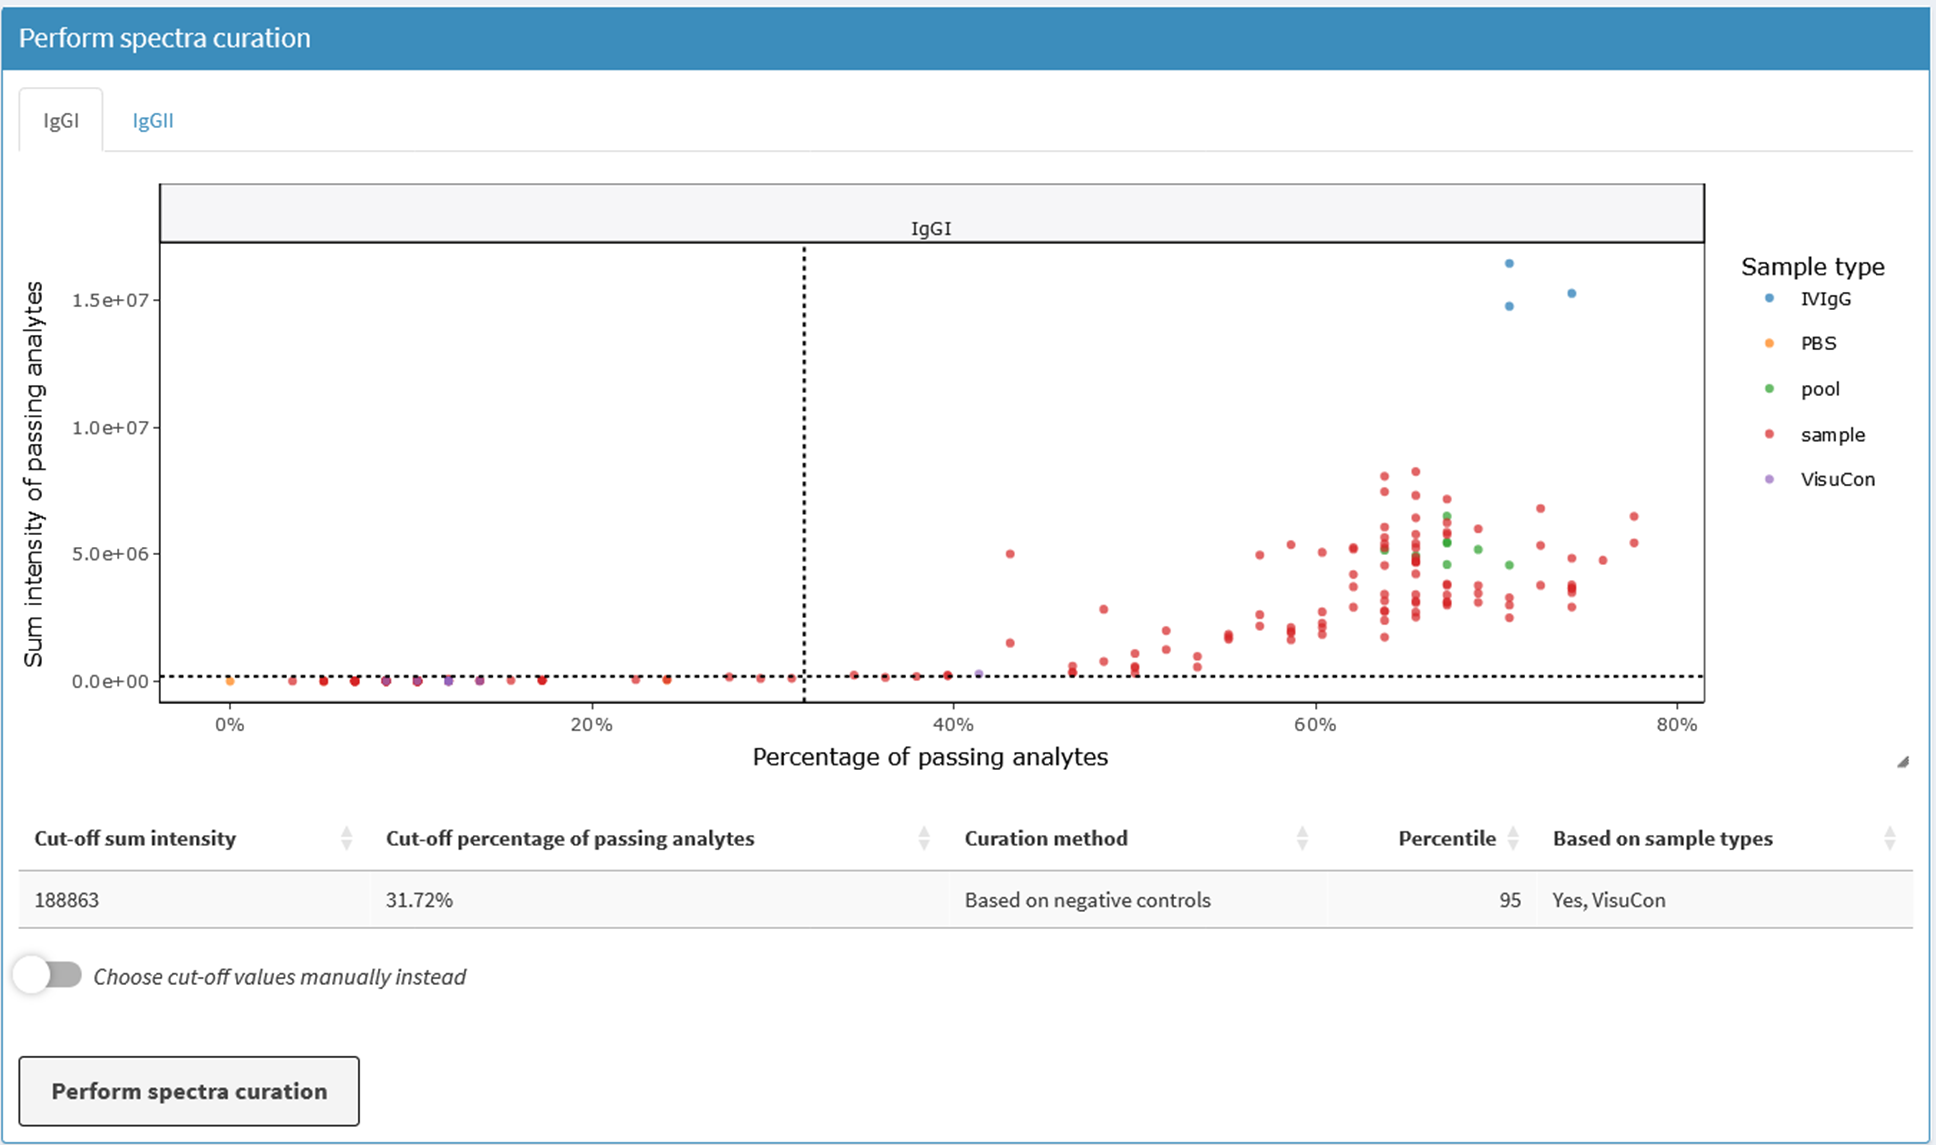
\includegraphics[scale=0.29]{perform_curation.png}
\end{center}



\newpage
\subsubsection{Curate spectra based on percentiles}
In this scenario, cut-off values are determined at a set percentile based on all measurements associated with a glycosylation site, with the option to exclude a selection of sample types from the calculation.
Using this method, a fixed proportion of all data (that of the lowest quality) will be excluded from further processing.

\begin{enumerate}[topsep=0pt, itemsep=0pt]
	\item Choose the percentile at which to set the cut-off values. 
	The default value is set to 5.
	\item Optionally, exclude certain sample types from the calculations.
	It is recommended to exclude all types of control samples.
	Excluded samples will still be curated based on the calculated cut-off values.
	\item Review the cut-off values in the \textsf{Perform spectra curation} box.
	\item When satisfied with the cut-offs, click on \menu{Perform spectra curation}.
\end{enumerate}


\subsection{Spectra curation results}
After performing spectra curation, an interactive plot displaying the results is generated. 
The plot shows the percentage of passing and failing spectra for each sample type per glycosylation site.
The reasons for failing curation are indicated by different colors.
For LaCyTools and SweetSuite output, the percentage of uncalibrated spectra is also displayed (this calibration step can be seen as a first-pass spectra curation).

\begin{center}
	
\includegraphics[scale=0.42]{curation_results.png}
\end{center}

Below the plots, three tables are shown displaying the following information:

\begin{itemize}[topsep=0pt, itemsep=0pt]
	\item Details of passing spectra per analyte.
	\item Overview of failed spectra.
	\item Details of failed spectra per analyte.
\end{itemize}

There is an option to download each of these tables as a \texttt{.xlsx} file, at the bottom of the page in the \textsf{Export results} box.




	\graphicspath{ {./images/4_Analyte_curation} }
\newpage

\section{Analyte curation}
The purpose of analyte curation is to decide which analytes can be measured at sufficient quality in the data set, thus improving the overall quality and reliability of the data.
There are four methods that can be used to perform analyte curation, as discussed below. 

\subsection{Based on percentages of passing spectra}
Analytes are curated based on the quality criteria that were chosen in the \menu{Spectra curation} tab.
An analyte passes curation if it meets the quality criteria in a percentage of spectra exceeding a chosen cut-off percentage.
The analyte is then used for total area normalization in all samples. 
The cut-off percentage can be set for each glycosylation site individually, or one cut-off can be applied to all of them.

There is an option to specify biological groups in the data. 
When used, an analyte that fulfills the quality criteria in a percentage exceeding the cut-off for at least one of the biological groups passes curation.
It will then be used for total area normalization in all samples, irrespective of their biological groups.
It is possible to ignore certain biological groups from this assessment (e.g., when dealing with a small number of samples in one of the groups).

Optionally, select sample types to ignore during the assessment, such as blanks and standards.
When curating per biological group, samples types that are not assigned to a biological groups are automatically excluded, even when they are not explicitly selected here.

\begin{optionalbox}
	If the data contains total and specific immunoglobulins, there is an option to exclude either one as a sample types during analyte curation.
	It is recommended to exclude total samples and base the curation solely on the specific samples.
\end{optionalbox}

One or two QC parameters may be excluded from the assessment entirely via the gears icon in the top-right corner of the \textsf{Method for analyte curation} box.

After performing curation, an interactive plot is generated for each glycosylation site.
Each analyte and charge state is represented by a bar in the plot, color-coded to indicate whether it passed curation.
If curation was performed per biological group, the plots are made for each group.

\begin{center}
	
\includegraphics[scale=0.55]{curation_results.png}
\end{center}


\newpage
Below the bar plots, a table listing all analytes is generated.
For each charge state, the table indicates whether the analyte passed curation, and there is a checkbox to include or exclude that analyte from further analysis.

Manual inclusion or exclusion of analytes should only be done when external information warrants this.

\begin{optionalbox}
	There is a toggle option to automatically include all charge states of analyte if at least one of the charge states passes curation.
	When using this option, strong interferences should be excluded (e.g., by manual inspection of raw data or LaCyTools/SweetSuite/Skyline output).
	Then, this likely increases accuracy at the expense of precision.
\end{optionalbox}


\subsection{Based on average QC parameters}
When the average values of the QC parameters fulfill the chosen requirements, then that analyte passes curation and is used for further analysis in all samples.
Average QC values can be calculated as either the mean or median.
An acceptable range must be set for the average mass accuracy.
For SweetSuite or LaCyTools data, a maximum value for the average IPQ and a minimum value for the $S/N$ must be specified.
For Skyline data, a minimum average IDP value and minimum average total area must be specified.

Like when curating based on the percentages of passing spectra, curation can be performed per biological group, and it is possible to exclude sample types from the assessment.

The curation results are visualized for each glycosylation site in a binary heatmap, with charge states on the $y$-axis and analytes on the $x$-axis.
The tiles are color-coded based on whether an analyte passed curation.
When hovering over the tiles, the average values for the QC parameters are displayed.

Below the heatmaps, the same checkbox table is generated as when performing curation based on the percentages of passing spectra. 

\begin{center}
	
\includegraphics[scale=0.75]{heatmap.png}
\end{center}



\newpage

\subsection{Per sample}
If an analyte meets the quality criteria in one sample, it is used for total area normalization in that sample. 
If the same analyte does not meet the criteria in some other sample, then it is not used for normalization in that particular sample.
The results from this curation method are not visualized, but a table containing checkboxes is again generated.

\subsection{Supply an analyte list}
\emph{This method should only be used if you performed analyte curation based on your data outside of GlycoDash.}

You can choose to supply an analyte list (as a \texttt{.xlsx} file or R object) that contains the names of all analytes that should be kept. 
This method does not distinguish between charge states: all charge states of the specified analytes will pass the curation.




	\graphicspath{ {./images/5_Normalized_data} }
\newpage

\section{Normalized data}
Following analyte curation, total area normalization is automatically conducted on the data per glycosylation site. 
A table displaying the normalized data is generated, including the following information:

\begin{itemize}[topsep=0pt, itemsep=0pt]
	\item Sample names
	\item Sample types
	\item Sample IDs
	\item Plate well positions (if applicable).
	\item The number of replicates for each sample ID.
	\item Metadata (if applicable).
	\item Columns showing the total spectrum intensities for per glycosylation site.
	\item For each analyte, a column displaying the relative abundance in percentages.
	Analytes associated to the same glycosylation site will collectively sum to 100\%.
\end{itemize}

\begin{optionalbox}
	Above the table, there is an option to normalize charge states separately instead of combining them per analyte.
\end{optionalbox}

The normalized data is visually represented in one or more heatmaps, with glycan compositions on the $x$-axis and glycosylation sites on the $y$-axis by default.
Each color in the heatmap corresponds to the median relative abundance for a specific glycopeptide, calculated across all samples.
There is an option to exclude sample types from this calculation.
If analyte curation was performed per biological group, there will be an option to separate heatmaps per biological group (enabled by default).
\begin{center}
	
\includegraphics[scale=0.42]{heatmap.png}
\end{center}

Alternatively, the individual samples can be plotted on the $y$-axis.
In this case, a heatmap is generated for each glycosylation site, with the ability to exclude sample types. 
If curation was performed per biological groups, the heatmaps can be generated per group.


	\graphicspath{ {./images/6_Protein_quantitation} }
\newpage

\section{Protein quantitation (optional)}
This option can be used when the samples contain one or more stable isotope labeled standards, such as SILuMAb for quantitation of antigen-specific IgG1.\footnote{See our technical note for details: \url{https://pubs.acs.org/doi/10.1021/acs.jproteome.4c00538}}

A \texttt{.xlsx} file containing the following columns is required:
\begin{itemize}[topsep=0pt, itemsep=0pt]
	\item \textsf{protein} - Name of the protein to be quantified using the natural/labeled pair.
	\item \textsf{natural} - Name of the natural glycosylation site (when quantifying based on glycopeptides), or the name of a natural non-glycosylated peptide \emph{as detected by GlycoDash} (see \nameref{data_import}).
	\item \textsf{labeled} - Name of the stable isotope labeled glycosylation site (when quantifying based on glycopeptides), or of the labeled non-glycosylated peptide \emph{as detected by GlycoDash} (see \nameref{data_import}).
	\item \textsf{standard\_ng} - The absolute amount of stable isotope labeled standard that was added to each sample, in nanograms (ng).
	This amount is assumed to be identical for all samples.
	\item \textsf{sample\_ul} - The volume of sample from which the proteins were isolated, in microliters ($\textmu$L). 
	This volume is assumed to be identical for all samples.
\end{itemize}

\begin{examplebox}
	Below is a screenshot of an example \texttt{.xlsx} file.
	\begin{center}
		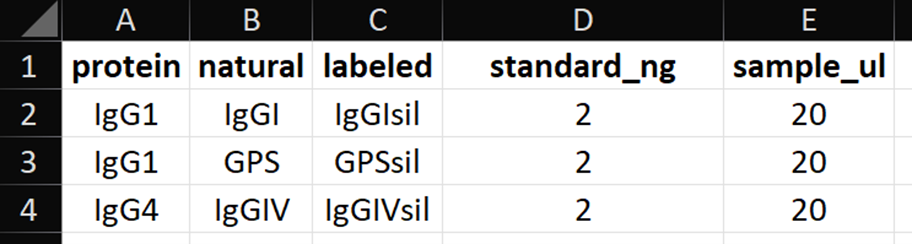
\includegraphics[scale=0.35]{example.png}
	\end{center}
	Here two proteins were quantified:
	\begin{itemize}[topsep=0pt, itemsep=0pt]
		\item \textsf{IgG1} was quantified based on glycopeptides and based on a non-glycosylated peptide.
		\begin{itemize}
			\item \textsf{IgGI} was the glycosylation site of natural \textsf{IgG1} glycopeptides.
			\textsf{IgGIsil} was the name of the glycosylation site of the labeled \textsf{IgG1} glycopeptides.
			\item \textsf{GPS} was the name of a natural non-glycosylated peptide, and \textsf{GPSsil} was the name of the corresponding labeled peptide.
		\end{itemize}
		\item \textsf{IgG4} was quantified based solely on glycopeptides, \textsf{IgGIV} representing the natural glycopeptides and \textsf{IgGIVsil} representing the labeled glycopeptides.
	\end{itemize}
\end{examplebox}

Quantitation using glycopeptides is based on the sum intensity ratio between the natural glycopeptides and the labeled glycopeptides.
Quantitation using non-glycosylated peptides is based on the intensity ratio between the natural peptide and the labeled peptide.

Quantities are reported as concentrations in the original sample in nanograms per millileter (ng/mL). 
\emph{Note that this may be a systematic underestimation if the standard is not added to the original sample but in a later step during the sample preparation.}

When more than one natural/labeled pair is specified for a protein, the median quantity is reported.
In the example above, \textsf{IgG1} was quantified based on both \textsf{IgGI/IgGIsil} and \textsf{GPS/GPSsil} ratios, giving two different quantities for each sample.
The reported quantity is the median of these two quantities.

\newpage
Correlation plots between the quantities based on the different pairs are generated, including a line of equality ($y = x$).
The closer data points are to this line, the more the two quantity calculations are in agreement.
Ideally, there should be a good correlation.
Otherwise, we suggest to investigate the validity of each natural/labeled pair.

Non-glycosylated peptides are not considered during spectral curation and analyte curation.
When non-glycosylated peptides are used for quantitation of a protein, the percentage of samples in which the peptide ions fulfill the three quality criteria is plotted.
For $S/N$ and IPQ (in the case of LaCyTools or SweetSuite data), or total area and IDP (Skyline data), the same criteria that were used for spectra and analyte curation are applied.
Because non-glycosylated peptides are often quantified without spectrum calibration, you may want to be more lenient when it comes to the acceptable mass error.
This acceptable mass accuracy range can therefore be set manually.
There is also an option to exclude sample types (e.g., blanks and negative controls) from the quality assessment.

\begin{center}
	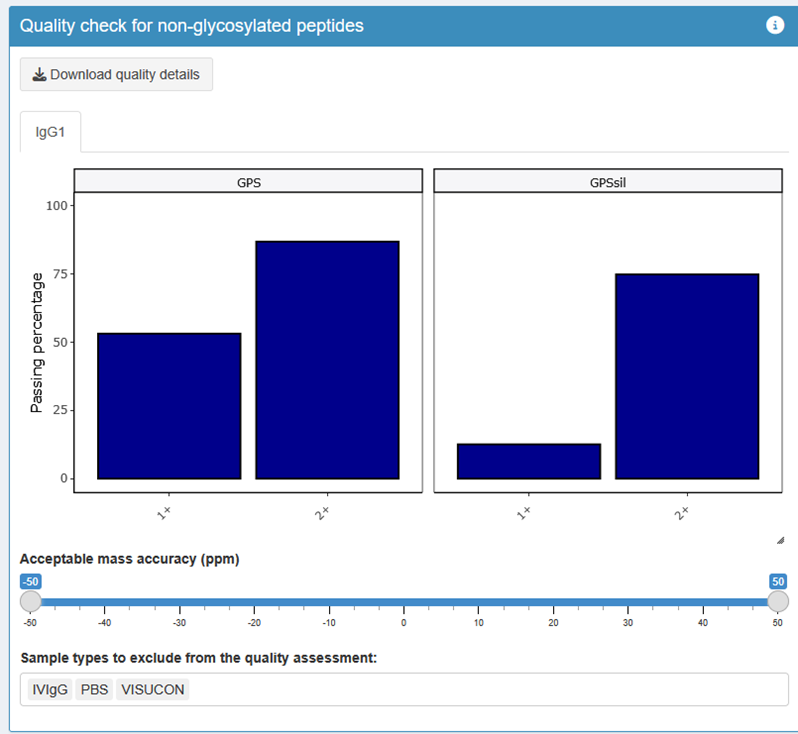
\includegraphics[scale=0.7]{peptide_qc.png}
\end{center}

If you conclude that a certain peptide or one of its charge states is of insufficient quality, it can be excluded from being used for quantitation under \textsf{Non-glycosylated peptide ions to exclude from the calculations}.






	\graphicspath{ {./images/7_Glycosylation_traits} }
\newpage

\section{Glycosylation traits (optional)}
Glycosylation traits can be calculated automatically for human IgG, IgA and IgM (including Joining Chain), and for mouse IgG.
These calculations rely on a reference list containing glycan compositions with known structures, listed in appendix \ref{glycan_compositions}.
If your curated data contains glycan compositions that are not listed there, there is an option to calculate glycosylation traits manually.

\subsection{Calculate traits automatically}
To calculate glycosylation traits automatically, start by selecting the type of glycans that are present in your data.
Then choose the traits that you wish to calculate.
For each desired trait, enter the glycosylation sites in your data for which they should be calculated.
Then click the \menu{Calculate traits} button.
\begin{center}
	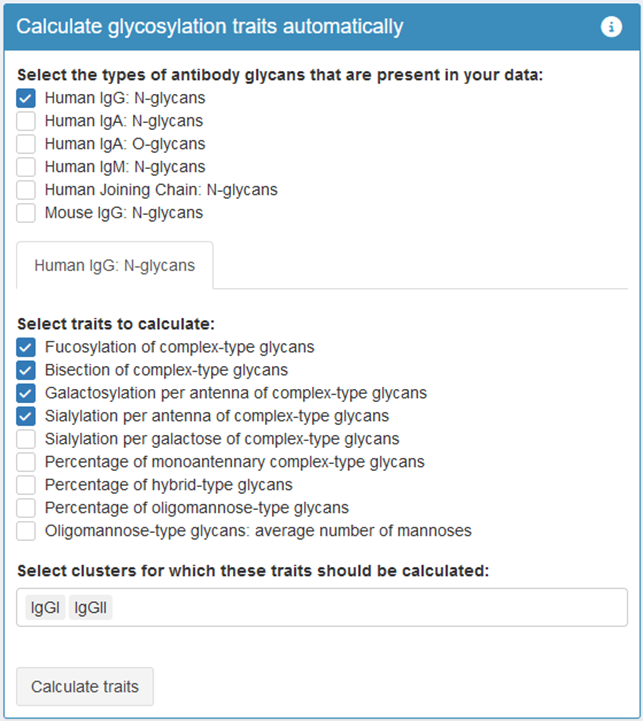
\includegraphics[scale=0.6]{traits_selection.png}
\end{center}

A table will be generated, displaying the formulas that were used for calculating the traits.
This table can be downloaded in \texttt{.xlsx} format.
In some cases, such as when a trait equals the same value for all samples, that trait will not be reported.
In such cases, a clear message will be shown in the table.

For each glycosylation site, the calculated trait values are plotted against total spectrum intensities as a sanity check.
Correlations between traits and spectrum intensities for standards (such as pools or VisuCon) indicate that differences in traits between samples are (partly) a technical artifact, rather than a biological effect. 


\newpage
\subsection{Calculate traits manually}
When your data is not suitable for calculating glycosylation traits automatically, there is an option to calculate them manually. 
To do so, start by creating a \texttt{.xlsx} file containing the following two columns:
\begin{itemize}[topsep=0pt, itemsep=0pt]
	\item \texttt{trait} - This column should contain the names of all the glycosylation traits that you want to calculate. \emph{Entries in this column should not contain any spaces}.
	\item \texttt{formula} - This column must contain the formulas that should be used for calculating the glycosylation traits. 
	Analyte names in the formulas should include information on the glycosylation site.
	An example of a valid formula (assuming the analytes are present in the data) is: \texttt{0.5*(H4N4F1 + H4N5F1) + H5N4F1}.
\end{itemize}

Upload this \texttt{.xlsx} file in the \textsf{Calculate custom glycosylation traits} box.

The traits will be calculated, and a table listing the trait names and corresponding formulas will be generated as a sanity check.

	\graphicspath{ {./images/8_Site_occupancy} }
\newpage

\section{Site occupancy (optional)}
GlycoDash will automatically detect the presence of non-glycosylated peptides in your data.
These are ignored during spectral and analyte curation. 
When a non-glycosylated peptide is present for a glycosylation site, this peptide can be used to calculate the corresponding site occupancy (e.g., when there are analytes \textsf{IgGI1H3N4F1}, \textsf{IgGI1H4N4F1}, etc. in your data, the analyte \textsf{IgGI1} without a glycan composition can be used).

\begin{wrapfigure}{R}{0.47\textwidth}
	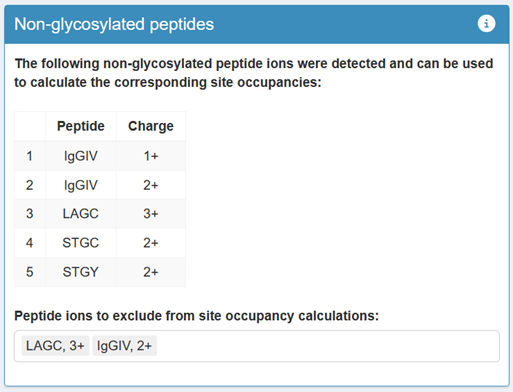
\includegraphics[scale=0.55]{peptides_table.png}
\end{wrapfigure}

The detected non-glycosylated peptides and their charge states are listed in a table, and corresponding site occupancies are automatically calculated.
You have the option to exclude ions from the site occupancy calculations, such as when the quality is insufficient (see below).
When you exclude all charge states for a peptide, the corresponding site occupancy is not calculated.

In the \textsf{Quality check} box, the quality of each detected peptide ion is visualized.
The percentage of samples in which the ion fulfills three quality criteria is plotted, with the option to exclude certain sample types from the assessment.
For $S/N$ and IPQ (SweetSuite and LaCyTools data), or total area and IDP (Skyline data), the same criteria that were used for spectral and analyte curation are applied.
Because non-glycosylated peptides are often quantified without internal calibration, you may want to be more lenient when it comes to the acceptable mass error. 
This value can therefore be set manually here.

\begin{center}
	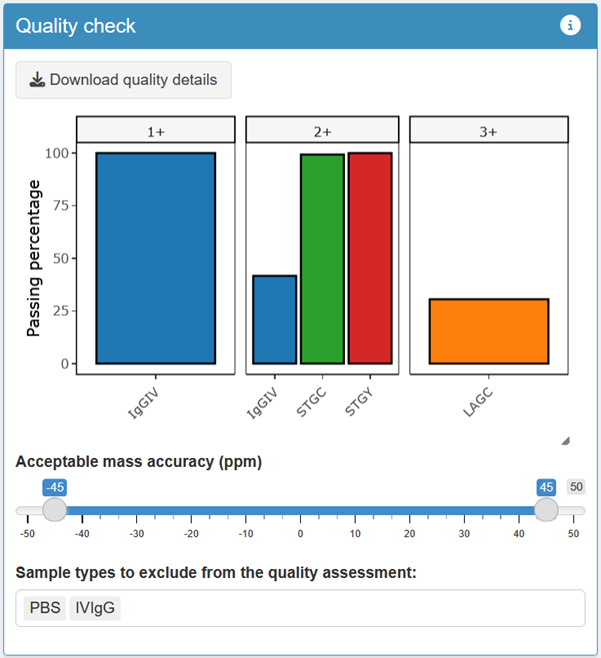
\includegraphics[scale=0.6]{peptides_quality.png}
\end{center}
	\graphicspath{ {./images/9_Repeatability} }
\newpage

\section{Repeatability (optional)}
For sample IDs that appear more than once in the dataset (e.g., \textsf{pool} or \textsf{VisuCon}), the repeatability of analyte relative abundances can be visualized. 
The repeatability for multiple sample IDs can be assessed by creating separate tabs using the \menu{Add a tab +} button in the top-right corner of the box.

In a tab, select the sample ID for which to visualize the repeatability.
Optionally, you toggle the option to visualize the repeatability per plate number.
Then click on \menu{Assess repeatability}.
An interactive bar plot is generated displaying the relative abundances of all analytes.
Error bars represent the [mean $\pm$ standard deviation (SD)] of each analyte.
The dots plotted over the bars indicate the relative standard deviations ($\text{RSD} = \text{SD} \times 100\%$).

\begin{center}
	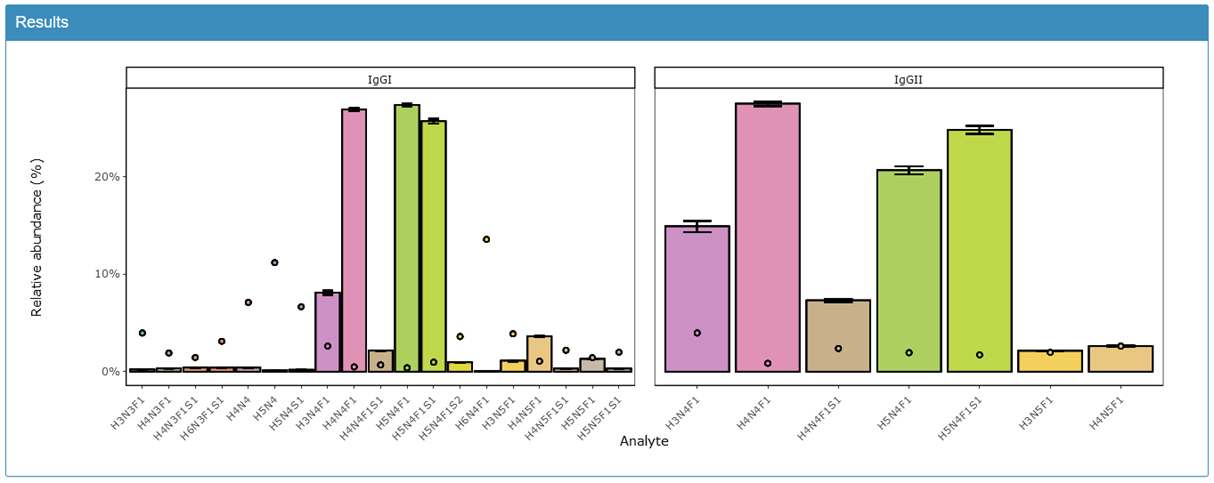
\includegraphics[scale=0.5]{repeatability.png}
\end{center}

When assessing the repeatability per plate, a table is presented showing median intra-plate variations, calculated as the median of the analyte RSDs on a plate.
At the bottom of the table, ther inter-plate variation is displayed, calculated as the mean of the intra-plate variations.

\begin{center}
	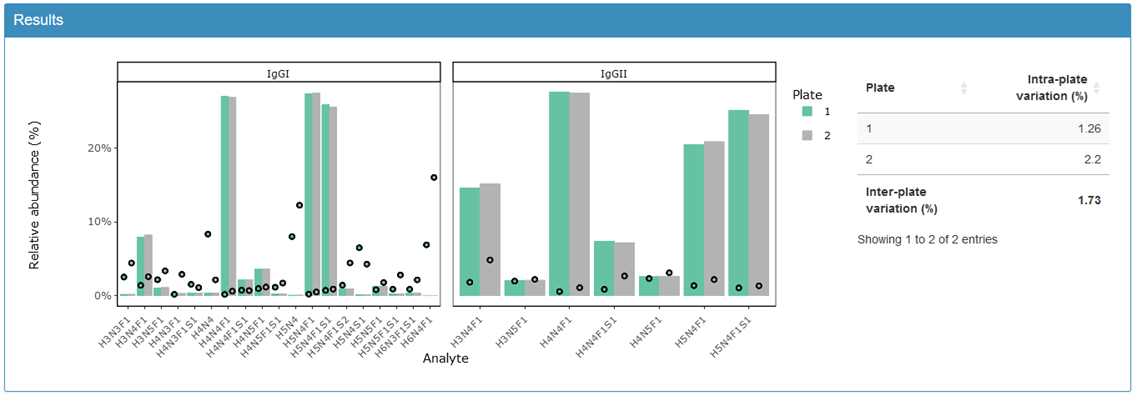
\includegraphics[scale=0.54]{repeatability_perplate.png}
\end{center}
	\graphicspath{ {./images/10_Data_exploration} }
\newpage

	\graphicspath{ {./images/11_Data_export} }
\newpage

\section{Data export}
In the \menu{Data export} tab you can download the processed data as in \texttt{.xlsx} format or as an R object. 

The processed data includes:

\begin{itemize}[topsep=0pt, itemsep=0pt]
	\item Sample names, sample types and sample IDs.
	\item Plate wells (if applicable).
	\item Uploaded metadata (if applicable).
	\item Sum intensities of all glycosylation sites.
	\item Relative abundances of all analytes.
	\item Calculated glycosylation traits, protein quantities and/or site occupancies (if applicable).
\end{itemize}

Additionally, you can download a data processing report in HTML format, which can be opened in any browser.
This report contains the GlycoDash version that was used, the names of uploaded files, choices that were made during each processing step, and all data visualizations.
The generated plots retain their interactivity in the HTML report.

There is also a section where you can make notes (e.g, about why you made certain choices during spectra or analyte curation).
These notes will be added to the bottom of the HTML report.

\begin{center}
	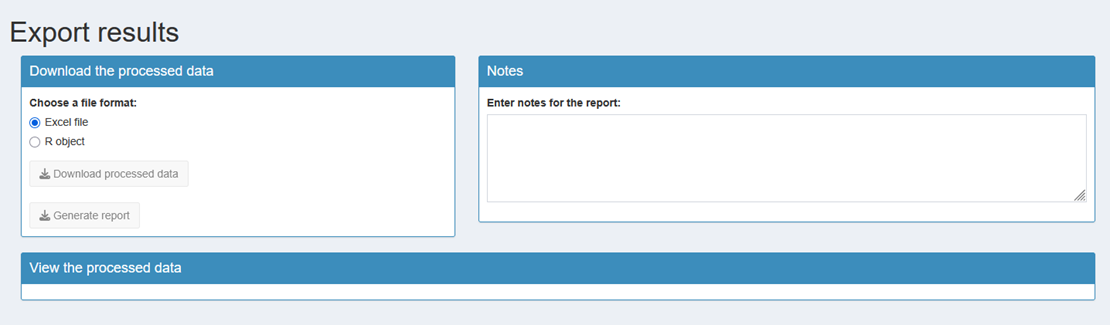
\includegraphics[scale=0.5]{export.png}
\end{center}
	
	% Appendices
	\newpage
	\begin{appendices}
	\graphicspath{ {./images/A1_Glycan_compositions} }

\section{Assumed glycan compositions}\label{glycan_compositions}
Below are lists of glycan compositions and their assumed structures.
These are used when automatically calculating glycosylation traits.

\subsection{Human IgG}

\newpage
\subsection{Human IgA}
\subsubsection*{IgA2 N47}
\subsubsection*{IgA1/2 N144/131}
\subsubsection*{IgA2 N205}
\subsubsection*{IgA1/2 N340/327}
\subsection*{IgA1 O-glycans}

\newpage
\subsection{Human IgM}
\subsubsection*{N46}
\subsubsection*{N209}
\subsubsection*{N272}
\subsubsection*{N279}
\subsubsection*{N440}

\newpage
\subsection{Human Joining Chain (JC)}

\newpage
\subsection{Mouse IgG}
	\end{appendices}
	
	
\end{document}
